% !TeX program = pdfLaTeX
\documentclass[12pt]{article}
\usepackage{amsmath}
\usepackage{graphicx,psfrag,epsf}
\usepackage{enumerate}
\usepackage{natbib}
\usepackage{textcomp}
\usepackage[hyphens]{url} % not crucial - just used below for the URL
\usepackage{hyperref}
\providecommand{\tightlist}{%
  \setlength{\itemsep}{0pt}\setlength{\parskip}{0pt}}

%\pdfminorversion=4
% NOTE: To produce blinded version, replace "0" with "1" below.
\newcommand{\blind}{0}

% DON'T change margins - should be 1 inch all around.
\addtolength{\oddsidemargin}{-.5in}%
\addtolength{\evensidemargin}{-.5in}%
\addtolength{\textwidth}{1in}%
\addtolength{\textheight}{1.3in}%
\addtolength{\topmargin}{-.8in}%

%% load any required packages here




\usepackage{booktabs}
\usepackage{pgf}
\usepackage{tikz}
\usepackage[ruled,vlined]{algorithm2e}
\usepackage[toc,page]{appendix}
\usepackage{longtable}
\hypersetup{ colorlinks=true, linkcolor=red, citecolor = blue, urlcolor=cyan, }
\newcommand*{\Appendixautorefname}{appendix}
\usepackage{float}
\floatplacement{figure}{t}
\usepackage[skip=0pt]{caption}
\usepackage{booktabs}
\usepackage{longtable}
\usepackage{array}
\usepackage{multirow}
\usepackage{wrapfig}
\usepackage{float}
\usepackage{colortbl}
\usepackage{pdflscape}
\usepackage{tabu}
\usepackage{threeparttable}
\usepackage{threeparttablex}
\usepackage[normalem]{ulem}
\usepackage{makecell}
\usepackage{xcolor}

\begin{document}


\def\spacingset#1{\renewcommand{\baselinestretch}%
{#1}\small\normalsize} \spacingset{1}


%%%%%%%%%%%%%%%%%%%%%%%%%%%%%%%%%%%%%%%%%%%%%%%%%%%%%%%%%%%%%%%%%%%%%%%%%%%%%%

\if0\blind
{
  \title{\bf Switching State Space Models for Interpreting Musical Dynamics}

  \author{
        Robert Granger \\
    Department of Statistics, Indiana University\\
      }
  \maketitle
} \fi

\if1\blind
{
  \bigskip
  \bigskip
  \bigskip
  \begin{center}
    {\LARGE\bf Switching State Space Models for Interpreting Musical Dynamics}
  \end{center}
  \medskip
} \fi

\bigskip
\begin{abstract}
In this paper, we attempt to illuminate a performer's musical intentions
using a Markov-switching state space model. Specifically, the model we
propose is designed for the dynamics of classical music. Unlike many
other models of trend estimation, this model requires the estimation of
a series of parameters. These parameters can be viewed as hidden musical
attributes of a performance that would not be revealed through the
calculation of simple statistics. For this analysis, we use dynamics
data of 46 different performances of Chopin's Mazurka Op. 68 No.~3. from
the Centre for the History and Analysis of Recorded Music (CHARM)
Mazurka Project.
\end{abstract}

\noindent%
{\it Keywords:} classical music, hidden Markov model
\vfill

\newpage
\spacingset{1.45} % DON'T change the spacing!

\def\algorithmautorefname{Algorithm}

\hypertarget{introduction}{%
\section{Introduction}\label{introduction}}

In this paper, we attempt to illuminate a performer's musical intentions
surrounding the dynamics of classical music. Through the use of a
Markov-switching state space model, the series of dynamics values within
a single performance are carefully smoothed with the goal of
differentiating the perceived intentions of the performer from the
observed dynamics found in the data. Classical music is different from
other types of music as a composer creates a piece, but many performers
may play it adding their own interpretation. While, the composer gives
some specific direction like the pitch of notes to play, the
instructions regarding dynamics are relatively vague. For example, when
performing a piece, a performer will observe a \emph{p} which stands for
\emph{piano}, indicating this section should be played ``softly''.
Meanwhile, an \emph{f} stands for \emph{forte} and indicates the given
section should be played ``loudly''. While we would expect the
\emph{forte} section to be played louder than the \emph{piano} section,
no direction is given on how softly or loudly the specified section
should be played. The performer may also attempt to ease into a
\emph{piano} section from a \emph{forte} section or they may want to
make a sudden change. These decisions are left to the interpretation of
the performer.

There are a variety of different trend estimating techniques, but we
propose using a Markov-switching state space model for two reasons.
First, the technique should incorporate actions found within a
performance. Often times, performers make dramatic changes in dynamics
to start a new section, something we want our model to identify, not
smooth out as noise. Likewise, this may extend to individual notes where
intentional emphasis is used by the performer. Using smoothing
techniques like a moving average or spline would ignore these key
elements. The second reason for using this type of model is that it
requires the estimation of certain parameters. These parameters offer
additional insight and can be viewed as hidden attributes of a
performance. Attributes found through simple calculation of averages and
variances would ignore the complexity of the decisions made during a
performance.

Similar analysis of modelling musical performances with Markov-switching
state space models has been performed on tempo data
\citep{mcdonald_markov-switching_2019,gu_modeling_2012}. When modeling
tempo, the expectation is for the performer to hold a constant tempo,
with some periods of potential speeding up or slowing down. This same
expectation cannot be said for the dynamics and thus requires a
different model setup. Although a Markov-switching state space model can
still be used, the difference comes in the selection of different
discrete states and parameter matrices. While Gu and Raphael did give
some attention to modeling dynamics, this paper looks to expand their
work.

\def\sectionautorefname{Section}

The paper procedes as follows: \autoref{Sec:model} begins with a general
description of Markov-switching state space models followed with
specific details regarding the states and the parameter matrices used to
model musical dynamics. \autoref{sec:analysis} explains the algorithm
used to evaluate the model and discusses results for several
performances. \autoref{sec:conclusion} briefly concludes with potential
uses of this model along with potential future areas of research.

\section{The Markov-Switching State Space Model}
\label{Sec:model}

State space models are commonly used to model time series observations
in the presence of hidden, continuous states. As a result of the state
space framework, the observations are viewed as independent conditional
on the hidden states whereas these hidden states will follow a vector
autoregressive process. Adding assumptions of linearity and normal error
produces what is commonly referred to as the general linear Gaussian
state space model \citep{durbin_time_2012}. It takes the form
\begin{equation}
  \begin{aligned}
    y_t &= C_t + D_tx_t + \epsilon_t, 
    & \epsilon_t & \sim N(0,G_t)\\
    x_{t+1} &= A_t + B_tx_t + \eta_t, 
    & \eta_t & \sim N(0,H_t), 
    & x_1 & \sim N(x_0,P_0) \\
  \end{aligned}
  \label{eq:statespacemod}
\end{equation} where the first part of \autoref{eq:statespacemod} is
known as the observation equation and the second part is known as the
state equation. The vector \(y_t\) consists of the known observations at
each time period, \(t\), whereas the vector \(x_t\) consists of the
unobserved, continuous states on which \(y_t\) is dependent. The
observation error, \(\epsilon_t\), and the state equation error,
\(\eta_t\), are assumed to be serially independent and independent of
each other.

In the typical state space framework, the matrices \(A_t\), \(B_t\),
\(C_t\), \(D_t\), \(G_t\), and \(H_t\) are allowed to vary across time
but are known. If there are a finite number of perceived structures for
these matrices, and the given structure is unknown at time, \(t\), a
Markov-switching state space model can be used. This model assumes there
are some underlying discrete states, \(s_t\), that transition over time
through a Markov process. Making this slight adjustment to
\autoref{eq:statespacemod} yields the following model which will be used
as a basic framework for modeling music dynamics.

\begin{equation}
  \begin{aligned}
    y_t &= C_t(s_t) + D_t(s_t)x_t + \epsilon_t, 
    & \epsilon_t & \sim N(0,G_t)\\
    x_{t+1} &= A_t(s_t) + B_t(s_t)x_t + \eta_t, 
    & \eta_t & \sim N(0,H_t), 
    & x_1 & \sim N(x_0,P_0) \\
  \end{aligned}
  \label{eq:switchstatemodel}
\end{equation}

When it comes to musical dynamics, rarely do musicians attempt to play
with the same dynamics or loudness throughout the entirety of a piece.
Most of the time we expect the musician to steadily change the loudness
from note to note; however, there may exist moments where the musician
deviates greatly from the trend with either louder or softer than usual
notes. A single note may be played more loudly because the performer is
specifically trying to add emphasis. Adding this emphasis may be on the
performer's own perogative or may be dictated by the piece with an
accent, ``\textbf{$>$}''. On the other hand, a single note appearing in
the data more softly is likely not part of the performer's intent. If a
note in the data is played more softly, it may be because the performer
missed a note or did not hit it as hard as intended. It could also be
something went wrong in the data creation step. Regardless, we do not
attempt to identify why the dynamics data indicates an unusually soft
note, but it is important to include this in our model for statistical
estimation purposes. We tried estimating without explicitly
incorporating these low sounds in the model, but the excessive
statistical noise caused the model to falsely indicate starts of new
smooth progressions. Therefore, in order to model the described
behavior, we propose the following four discrete states:

\begin{list}{}{}

\item[$s^1$:] The musician selects a new value for loudness.

\item[$s^2$:] The musician continues the dynamics in a steady way.

\item[$s^3$:] The musician plays a single note more loudly.

\item[$s^4$:] The musician plays a single note more softly.

\end{list}

The observation, \(y_t\) is the univariate loudness of the note at each
time period, \(t\). In order to allow the dynamics to progress steadily,
the continuous hidden states, \(x_t\), follow a process that allows for
piece-wise quadratics. At each time period, \(x_t\), is a vector of
length three, \[x_t^\prime = (x^0_t, x^1_t, x^2_t), \] where \(x^0_t\)
is the loudness, \(x^1_t\) is the first order difference, and \(x^2_t\)
is the second order difference. The aim is to maintain this smooth
progression even when the musician plays a single note more loudly or
softly. The states \(s^3\) and \(s^4\) are therefore implemented by
adding a constant in the observation equation as opposed to changing the
state equation. The model is similar to that proposed in
\cite{gu_modeling_2012}, but extended to include these additional
states. \autoref{tab:parmats} shows the parameter matrices for the four
states.

\begin{table}
\caption{Parameter matrices for the switching state space model.\label{tab:parmats}}
\centering
\begin{tabular}[h!]{@{}ccccccccc@{}}
\toprule
%&&&\multicolumn{3}{c}{Parameter Matrices}\\
  \multicolumn{2}{c}{States} &\phantom{a}& \multicolumn{6}{c}{Parameter Matrices}\\
  \cmidrule{1-2} \cmidrule{4-9}
  \multicolumn{2}{c}{$S$}&& $A$ & $B$ & $C$ & $D$ & $G$ & $H$ \\
  \midrule
  \multicolumn{2}{c}{$s^1$} && $\begin{pmatrix} \mu_0 \\ \mu_1 \\ \mu_2 \end{pmatrix}$ & $\begin{pmatrix} 0&0&0 \\ 0&0&0 \\ 0&0&0 \end{pmatrix}$ & 0 & $\begin{pmatrix} 1&0&0 \end{pmatrix}$ & $\sigma_\epsilon^2$ & $\begin{pmatrix} \sigma_0^2&0&0 \\ 0&\sigma_1^2&0 \\ 0&0&\sigma_2^2 \end{pmatrix}$\\
  \\
  \multicolumn{2}{c}{$s^2$} && $\begin{pmatrix} 0 \\ 0 \\ 0 \end{pmatrix}$ & $\begin{pmatrix} 1&1&0 \\ 0&1&1 \\ 0&0&1 \end{pmatrix}$ & 0 & $\begin{pmatrix} 1&0&0 \end{pmatrix}$ & $\sigma_\epsilon^2$ & $\begin{pmatrix} 0&0&0 \\ 0&0&0 \\ 0&0&0 \end{pmatrix}$\\
  \\
  \multicolumn{2}{c}{$s^3$} && $\begin{pmatrix} 0 \\ 0 \\ 0 \end{pmatrix}$ & $\begin{pmatrix} 1&1&0 \\ 0&1&1 \\ 0&0&1 \end{pmatrix}$ & $\mu_c$ & $\begin{pmatrix} 1&0&0 \end{pmatrix}$ & $\sigma_\epsilon^2$ & $\begin{pmatrix} 0&0&0 \\ 0&0&0 \\ 0&0&0 \end{pmatrix}$\\
  \\
  \multicolumn{2}{c}{$s^4$} && $\begin{pmatrix} 0 \\ 0 \\ 0 \end{pmatrix}$ & $\begin{pmatrix} 1&1&0 \\ 0&1&1 \\ 0&0&1 \end{pmatrix}$ & $\mu_e$ & $\begin{pmatrix} 1&0&0 \end{pmatrix}$ & $\sigma_\epsilon^2$ & $\begin{pmatrix} 0&0&0 \\ 0&0&0 \\ 0&0&0 \end{pmatrix}$\\

\bottomrule
\end{tabular}
\end{table}

The final part of the switching state space model is designing the
Markov process for transitioning between the discrete states which is
displayed in \autoref{fig:transmat}. The first state, \(s^1\), allows
for the selection of a new loudness which then transitions into the
smooth progresson state, \(s^2\), with probability 1. When arriving in
\(s^2\), the next time period's discrete state can be any of the
possible states including itself. If in this progression, we move to a
sudden loud note, \(s^3\), or a sudden soft note, \(s^4\), then we have
the opportunity to continue the smooth progression, \(s^2\), or start a
new smooth progression, \(s^1\). It is not permissible though to
immediately then play another sudden loud or soft note.

In total, there are 13 unknown parameters, \(\theta \in \Theta\), spread
across 4 different discrete states, \(s^i \in S\), through \(T\) time
periods. A summary of the parameters to be estimated are:
\(\Theta = \{\mu_c, \mu_e, \sigma^2_\epsilon, \mu_0, \mu_1, \mu_2, \sigma^2_0, \sigma^2_1, \sigma^2_2, p_{21}, p_{23}, p_{24}, p_{41}\}\).
Note this vector contains only four probabilities. With four states, the
transition matrix could potentially have up to twelve probabilities
requiring estimation; however, because of the restrictions placed on the
possible transitions, this number is reduced to four. In the next
section, we discuss finding smoothed estimates of the dynamics which
requires estimation of these parameters along with the continuous and
discrete states.

\begin{figure}[tb!]
\caption{Transition diagram. \label{fig:transmat}}
  \centering
  \tikzstyle{switch}=[rectangle,
  thick, minimum size=1cm, draw=black]
  \begin{tikzpicture}[>=latex,text height=1.5ex,text depth=0.25ex]
    \matrix[row sep=0.25cm,column sep=.5cm] {
      &&& \node (S1) [switch] {$s^1$};&&& \\
      \\ \\ \\ \\ \\ \\
      &&& \node (S2) [switch] {$s^2$};&&& \\
      \\ \\ \\ \\ \\ \\
      &\node (S3) [switch] {$s^3$}; &&&& \node (S4) [switch] {$s^4$};\\
    };
    \path[->]
    (S1) edge [bend right] node [left] {1}(S2)
    (S2) edge [bend right] node [right] {$p_{21}$}(S1)
    (S2) edge [loop above] node [left] {}(S2)
    (S2) edge [bend right] node [right] {$p_{23}$}(S3)
    (S2) edge [bend right] node [right] {$p_{24}$}(S4)
    % (S3) edge [bend left] node [left] {$p_{31}$}(S1)
    (S3) edge [bend right] node [left] {1}(S2)
    (S4) edge [bend right] node [right] {$p_{41}$}(S1)
    (S4) edge [bend right] node [left] {}(S2);
  \end{tikzpicture}
\end{figure}

\section{Evaluating the Model}
\label{sec:analysis}

Evaluation of the model requires the estimation of the parameters,
\(\theta \in \Theta\); the discrete states, \(\{s_t\}^T_{t=1}\); and the
continuous hidden states \(\{x_t\}^T_{t=1}\). These estimates are
obtained using only the assumptions and structure of the model along
with the observed dynamics, \(\{y_t\}^T_{t=1}\). Once these estimates
are obtained, we then compute predicted values, \(E[y_t|...]\), which
can be thought of as the performer's intended dynamics. Hence, the aim
in estimating the intended dynamics is attempting to remove
\(\epsilon_t\), which can be seen as unintended deviations from the
desired loudness.

\subsection{The Algorithm}

When the parameter values, \(\theta_i \in \Theta\), and the discrete
states, \(\{s_t\}^T_{t=1}\), are known, the Kalman filter
\citep{kalman_new_1960} can be used to find estimates of the continuous
hidden states, \(\{x_t\}_{t=1}^T\), along with the likelihood. While the
Kalman filter provides an easy way to compute the likelihood, the
estimate of \(x_t\) is obtained using only observations coming before
time \(t\). In order to use all information, we implement the Kalman
smoothing algorithm introduced in \citep{rauch_maximum_1965}. This
algorithm provides an estimate, \(\hat{x_t} = E[x_t|y_1,...y_T]\), which
can be used to compute a fitted or ``smoothed'' value, \(\hat{y_t}\).

The Kalman smoother provides a closed form solution to obtaining the
maximum likelihood estimates of our continuous hidden states, but what
if the discrete states, \(\{s_t\}^T_{t=1}\), are unknown? We can obtain
the most likely set of discrete states by simply running the Kalman
smoother algorithm on every possible combination of discrete states and
choosing the set of discrete states that yields the largest likelihood.
This may work if the number of discrete states and/or time periods is
small; however, the number of state combinations to check may be large
and can be computed as \(|\{s^i \in S\}|^T\). For example, the music
dynamics model presented in the previous section has four discrete
states and the piece to be evaluated, Chopin's Mazurka Op.~68 No.~3, has
231 notes. This brings the grand total of state combinations to check to
\(4^{231}\approx1.19\times 10^{139}\). Of course, many of these state
combinations could be removed due to 0 likelihood given the restrictions
on the state transitions, but even with this taken into account, the
number of state combinations is far too large. To overcome this issue,
we use the Discrete Particle Filter as described in
\cite{mcdonald_markov-switching_2019}. We begin by estimating the
partial likelihood iteratively through time at each of the possible
discrete state paths using the Kalman Filter. Each of these paths is
known as a particle with only the previous states and partial likelihood
being saved. This process would still require checking all
\(|\{s^i \in S\}|^T\) paths, so to get around this, we implement the
greedy search algorithm called Beam Search. This search algorithm
requires selecting a maximum number of particles to save at each time
iteration and discards the rest.

\begin{figure}[tb!]
  \centering
  \tikzstyle{switch}=[rectangle,
  thick, minimum size=0.5cm, draw=black]
  \begin{tikzpicture}[>=latex,text height=1.5ex,text depth=0.25ex]
    \matrix[row sep=0.25cm,column sep=.75cm] {
      \node (S1) [switch] {$s_1$}; &&\node (S4) [switch] {$s_1s_1$};&& \node (S7) [switch] {$s_1s_1$}; && \node (S8) [switch] {$s_1s_1s_1$}; && \node (S9) [switch] {$s_1s_1s_1$}; &&\\
      \\
      && && && \node (S13) [switch] {$s_1s_1s_2$};\\
      \\
       &&\node (S3) [switch] {$s_1s_2$}; && \node (S10) [switch] {$s_1s_2$}; && \node (S14) [switch] {$s_1s_2s_1$}; && \node (S20) [switch] {$s_1s_2s_1$}; \\
      \\ 
             && &&  && \node (S15) [switch] {$s_1s_2s_2$}; && \node (S21) [switch] {$s_2s_2s_2$}; \\
      \\
      \node (S2) [switch] {$s_2$}; &&\node (S5) [switch] {$s_2s_1$};&&\node (S11) [switch] {$s_2s_1$};&& \node (S16) [switch] {$s_2s_1s_1$}; && \node (S22) [switch] {$s_2s_1s_1$}; \\
      \\
      && && && \node (S17) [switch] {$s_2s_1s_2$};&&\node (S23) [switch] {$s_2s_1s_2$};
      \\ 
       &&\node (S6) [switch] {$s_2s_2$};&&\node (S12) [switch] {$s_2s_2$};&& \node (S18) [switch] {$s_2s_2s_1$};\\
      \\
      &&&&&& \node (S19) [switch] {$s_2s_2s_2$}; &&\\
      \\
      \hline
      \\
      \\
      $t=1$ && && \hspace{12px} $t=2$ && && \hspace{52px} $t=3$  \\
    };
    \path[->]
    (S1) edge (S3)
    (S7) edge (S8)
    (S7) edge (S13)
    (S8) edge [dashed] (S9)
    (S10) edge (S14)
    (S10) edge (S15)
    (S11) edge (S16)
    (S11) edge (S17)
    (S4) edge [dashed] (S7)
    (S1) edge (S4)
    (S2) edge (S5)
    (S12) edge (S18)
    (S12) edge (S19)
    (S3) edge [dashed] (S10)
    (S5) edge [dashed] (S11)
    (S6) edge [dashed] (S12)
    (S14) edge [dashed] (S20)
    (S15) edge [dashed] (S21)
    (S16) edge [dashed] (S22)
    (S17) edge [dashed] (S23)
    (S2) edge (S6);
  \end{tikzpicture}
  \caption{Discrete Particle Filter with 2 discrete states and capping the maximum number of stored particles at 5 for each time iteration. \label{fig:dpf}}
\end{figure}

\autoref{fig:dpf} illustrates this concept with 2 discrete states and
the maximum number of particles set at 5. There are four possible state
paths to check when passing from \(t=1\) to \(t=2\) which is less than
the maximum particle number so all four paths are saved. When moving
from \(t=2\) to \(t=3\), the number of paths increases to 8. Since only
5 paths are allowed, three of these paths must be dropped and will no
longer be considered as possible solutions. In order to decide which
paths are to be saved a sampling procedure must be performed. One
sampling procedure proposed by \citep{tugnait_detection_1982} is to
simply keep the paths that have the highest likelihood. Another sampling
procedure proposed by \citep{akashi_random_1977} is to randomly sample
one particle out of the total number of states descended from each of
the \(t-1\) particles in proportion to their respective likelihoods.
\citep{fearnhead_-line_2003} proposes another stochastic approach but
one that minimizes the expected mean squared error between the
approximated distribution and the true distribution's probabilities.
This approach determines a threshold value such that all particles with
likelihood above this value are kept and the remaining particles to be
kept are chosen at random with probability equal to their respective
likelihoods. Once a sampling technique is selected and the procedure is
implemented through all time points, a sample of discrete state
sequences is saved the size of the beam width. Since the goal of this
paper is to find the most likely sequence of discrete states, the one
with the highest likelihood is selected.

\begin{algorithm}[t]
 \caption{Solving Music Dynamics Model\label{alg:masteralgorithm}}
\SetAlgoLined
 \textbf{Input} Y, a vector of observed dynamics\;
 \textbf{Initialize} $\Theta$\;
 \While{(Stopping Criteria)}{
 Create Matrices A, B, C, D, G, H at each $t$ for each $s^i \in S$\;
 Implement Discrete Particle Filter\;
 Compute the log-likelihood: \hspace{2px} $l(Y|\Theta,S) + l(S|\Theta) + l(\Theta)$\;
 Update $\Theta$ via Nelder-Mead Optimization or SANN\;
 }
\end{algorithm}

The final step is estimating the model parameters, \(\Theta\), that
maximize the likelihood. This is a difficult task as this model presents
a couple of problems: 1) many of the parameters are constrained as
variances need to be positive and the probabilities of leaving the same
state should sum to 1 while also being constrained between 0 and 1; 2)
there are many local maxima making finding a global maxima difficult. To
help alleviate these concerns, we can include Bayesian priors on our
parameters. Using carefully selected priors allows us to steer the
algorithm away from impossible solutions and direct it toward more
desired solutions. These issues also lead us to carefully consider our
optimization technique. We will use two different methods. The first is
the Nelder-Mead algorithm which can find local maxima for unconstrained
multidimensional problems without the need for derivative computation
\citep{nelder_simplex_1965}. The second is the Simulated Annealing
(SANN) algorithm which is commonly used when dealing with problems with
many local maxima in order to estimate the global maxima. Neither of
these methods are perfect at avoiding a local maximum and hence the
selection of initial values plays an important role. To overcome this
challenge, we will select a variety of different starting points drawn
randomly from the Bayesian priors.

\vspace{10px}

\autoref{alg:masteralgorithm} displays the complete procedure. The
solution to this model was found using software R
\citep{r_core_team_r_2019}. The Nelder-Mead and SANN methods are
performed using the package \texttt{optimr} by \cite{nash_optimr_2019}.
The discrete particle filter was implemented by extending the package
\texttt{dpf} by \cite{mcdonald_dpf_2020}.

\subsection{Results for Chopin's Mazurka Op.\ 68 No.\ 3}

\begin{table}[t]
  \caption{Informative prior distributions for Chopin's Mazurka Op.\ 68 No.\ 3}
  \centering
  \begin{tabular}{@{}rcll@{}}
    \toprule
    Parameter & \phantom{a} & Distribution & Prior Mean \\
    \midrule
    $\mu_c$ & $\sim$ & Gamma$(100,\ 0.1)$ & 10\\
    $\mu_e$ & $\sim$ & -Gamma$(100,\ 0.1)$ & -10\\
    $\sigma^2_{\epsilon}$ & $\sim$ & Gamma$(10,\ 0.5)$ & 5\\
    $\mu_{0}$ & $\sim$ & Normal$(\overline{Y},\ 10)$ & $\overline{Y}$\\
    $\mu_{1} $ & $\sim$ & Normal$(0,\ 0.25)$ & 0\\
    $\mu_{2} $ & $\sim$ & Normal$(0,\ 0.25)$ & 0\\
    $\sigma^2_{0} $ & $\sim$ & Gamma$(10,\ 1)$ & 10 \\
    $\sigma^2_{1} $ & $\sim$ & Gamma$(3,\ 1)$ & 3 \\
    $\sigma^2_{2} $ & $\sim$ & Gamma$(3,\ 1)$ & 3 \\
    $p_{2,\cdot}$ & $\sim$ & Dirichlet$(5,\ 85,\ 5,\ 5)$ & 0.05, 0.85, 0.05, 0.05 \\
    % $p_{3,\cdot}$ & $\sim$ & Beta$(2,\ 8)$ & 0.20\\
    $p_{4,\cdot}$ & $\sim$ & Beta$(2,\ 8)$ & 0.20\\
    \bottomrule
  \end{tabular}
  \label{tab:priors}
\end{table}

The model was estimated using observed dynamics from forty-six different
performances of Chopin's Mazurka Op.~68 No.~3. This data was reverse
conducted (created) by Craig Sapp using Andrew Earis's Expression
Algorithm software. The software and data can be found on the website
for the Centre for the History and Analysis of Recorded Music (CHARM)
Mazurka Project \citep{charm_centre_2009}. The technique used to create
the data is described in detail in Andrew Earis's paper ``An algorithm
to extra expressive timing and dynamics from piano recordings''
\citep{earis_algorithm_2007}.

To implement \autoref{alg:masteralgorithm} on dynamics data from
performances of Chopin's Mazurka Op.~68 No.~3, we must make a few
specific decisons. First, we choose prior distributions applicable
specifically to Chopin's Mazurka Op.~68 No.~3, which can be found in
\autoref{tab:priors}. Secondly, regarding the Discrete Particle Filter,
we selected to keep up to 500 particles with the sampling criterion of
keeping the largest likelihoods. Lastily, since there are many local
minima, we used 10 different starting points drawn randomly and
independently from each of the prior distributions for each optimization
technique (both Nelder-Mead and SANN).

\begin{figure}
\centering
\includegraphics{Dynamics-Model_files/figure-latex/exampletable-1.pdf}
\caption{\label{fig:exampletable}Interpreted Dynamics from selected
performances of Chopin's Mazurka Op. 68 No.~3. The black line traces the
observed dynamics while the colored dots are the smoothed interpreted
dynamics.}
\end{figure}

Graphical representations for the performances of Jean-Marc Luisada in
1991 and Arthur Rubinstein in 1966 are shown in
\autoref{fig:exampletable}. These along with plots of the other
forty-four performances can be found in \autoref{appendixd}. The black
line traces the observed dynamics for each note across musical time as
given by the score. The colored dots are used to differentiate the 4
possible discrete states and show the interpreted musical dynamics for
each note. The background is shaded based on musical directions given by
the composer in the score. Notice with these performances, the model
often seems to start a new smooth progression when the composer gives
direction about the dynamics. There are occasions where this is not
always the case. Notice that Luisada appears to smoothly adjust the
dynamics from the second \emph{piano} section into the
\emph{poco piu vivo} section and again when transitioning from the final
\emph{forte} section to the final \emph{piano} section. Similarly,
Rubinstein also smoothly transitions but he does this between the first
\emph{forte} section into the only \emph{fortissimo} section. These
unscripted parts of the performance are what we hope to discover as they
allow us to contrast and compare each performance.

\begin{table}

\caption{\label{tab:table3}Parameter Estimates for Selected Performances of Chopin's Mazurka Op.68 No.3\label{tab:parameterestimatesrichter}}
\centering
\begin{tabular}[t]{lrrrrrrrrr}
\toprule
  & $\mu_c$ & $\mu_e$ & $\sigma^2_\epsilon$ & $\mu_0$ & $\mu_1$ & $\mu_2$ & $\sigma^2_0$ & $\sigma^2_1$ & $\sigma^2_2$\\
\midrule
\rowcolor{gray!6}  Block 1995 & 8.812 & -9.777 & 4.946 & 17.036 & 0.121 & -0.075 & 15.546 & 0.215 & 0.006\\
Grinberg 1951 & 10.038 & -9.342 & 5.906 & 19.381 & 0.553 & -0.094 & 16.676 & 0.396 & 0.006\\
\rowcolor{gray!6}  Hatto 1993 & 9.871 & -10.167 & 6.524 & 10.913 & 0.050 & -0.042 & 9.900 & 0.359 & 0.002\\
Luisada 1991 & 10.455 & -9.949 & 13.068 & 27.312 & -0.165 & -0.110 & 12.098 & 1.612 & 0.067\\
\rowcolor{gray!6}  Richter 1976 & 9.541 & -10.499 & 4.399 & 23.422 & -0.346 & -0.001 & 16.294 & 0.260 & 0.003\\
\addlinespace
Rubinstein 1966 & 10.771 & -10.065 & 8.091 & 12.840 & 0.470 & -0.033 & 17.045 & 0.401 & 0.000\\
\rowcolor{gray!6}  Sofronitsky 1949 & 9.944 & -10.538 & 9.154 & 27.735 & -0.234 & -0.070 & 13.768 & 0.659 & 0.019\\
\bottomrule
\end{tabular}
\end{table}

\begin{table}

\caption{\label{tab:table3ext}Probability Estimates for Selected Performances of Chopin's Mazurka Op.68 No.3\label{tab:probestimatesrichter}}
\centering
\begin{tabular}[t]{lrrrr}
\toprule
  & $p_{21}$ & $p_{23}$ & $p_{24}$ & $p_{41}$\\
\midrule
\rowcolor{gray!6}  Block 1995 & 0.101 & 0.027 & 0.025 & 0.124\\
Grinberg 1951 & 0.067 & 0.027 & 0.027 & 0.077\\
\rowcolor{gray!6}  Hatto 1993 & 0.056 & 0.070 & 0.067 & 0.053\\
Luisada 1991 & 0.037 & 0.020 & 0.024 & 0.136\\
\rowcolor{gray!6}  Richter 1976 & 0.046 & 0.017 & 0.051 & 0.044\\
\addlinespace
Rubinstein 1966 & 0.034 & 0.017 & 0.023 & 0.214\\
\rowcolor{gray!6}  Sofronitsky 1949 & 0.060 & 0.015 & 0.019 & 0.101\\
\bottomrule
\end{tabular}
\end{table}

Analyzing the graphical representations of each performance have the
benefit of illuminating complexities within a performance but may be
cumbersome when attempting to compare and contrast many performances.
Instead, we analyze the parameter and transition probability values,
\(\Theta\). All estimated values for the 46 performances can be found in
\autoref{appendixa} and \autoref{appendixb}. For the reader's
convenience, the parameter estimates for performances discussed in this
section can be found in \autoref{tab:parameterestimatesrichter} and
\autoref{tab:probestimatesrichter}. Along with the tables of estimated
parameters, we also supply density plots of the estimated parameters.
These density plots show the distribution of the estimated parameters
and should not be mistaken for the estimated posterior distributions for
some performance.

\begin{figure}
\centering
\includegraphics{Dynamics-Model_files/figure-latex/denseplots-1.pdf}
\caption{\label{fig:densityplots}Density Plots of Estimated Parameters
for 46 Performances of Chopin's Mazurka Op. 68 No.~3.}
\end{figure}

We analyze the density plots in order to get a better understanding of
the distribution of the parameters. We begin with a look at the
estimated parameters, \(\mu_{0}\) and \(\mu_1\). The parameter \(\mu_0\)
can be interpreted as the most likely starting point for each smoothed
quadratic section. Joyce Hatto's 1993 performance is estimated to have
the lowest average starting point with \(\mu_0=\) 10.913 and Vladimir
Sofronitsky's 1949 performance is estimated to have the highest average
starting point with \(\mu_0=\) 27.74. The average of all the \(\mu_0\)'s
across all 46 performances is \texttt{19.148}.
\autoref{fig:densityplots} displays the density plot of \(\mu_0\) which
reveals the distribution of \(\mu_0\)'s is fairly symmetric but with
more concentration around the mean than the normal distribution. The
parameter \(\mu_1\) can be interpreted as the average initial change in
the dynamics of a performance. As long as \(\mu_2\) is small relative to
\(\mu_1\) or if they both have the same sign, this change will
persistent through each smoothed quadratic section. The parameter
estimates for these performances range from a low of -0.346 in
Sviatoslav Richter's 1976 performance to a high of 0.553 in Maria
Grinberg's 1951 performance. From the density plot for \(\mu_1\), the
distribution of the estimated parameters appears roughly normal with a
mean equal to \texttt{0.103}. The mean being greater than zero indicates
that, on average, performers tend to (at least initially) increase the
volume through each smoothed quadratic section.

In order to get a fuller understanding of the parameters, we compare the
estimated parameters in Luisada's 1991 performance with Rubinstein's
1966 performance. Luisada's 1991 performance has \(\mu_0 = 27.312\),
\(\mu_1=-0.165\), and \(\mu_2=-0.110\) indicating that he typically
starts loudly and then softens. On the other hand, Rubinstein's
performance has \(\mu_0 = 12.840\), \(\mu_1=0.470\) and
\(\mu_2=-0.033\), indicating that he typically starts each smoothed
section more softly and then gets louder. Taking an average across all
note dynamics for the Luisada 1991 and Rubinstein 1966 performances
yields \texttt{17.33} and \texttt{20.98}, respectively. While it is
interesting to know that Rubinstein's 1966 was louder, on average, than
Luisada's 1991 performance, we can see that without modeling the
performer's intentions, interesting details are being missed. We also
analyze the variance within each performance. Calculating the overall
variation of note dynamics for the Luisada 1996 performance reveals a
variance of \texttt{48.39}. Calculating the overall note dynamics of the
Rubinstein 1996 performance reveals more homogeneity with a variance of
\texttt{31.84}. Although the variation in note dynamics is higher for
the Luisada 1996 performance, we observe through modelling the
performer's intentions that Luisada typically has less variation in the
starting dynamics of each piece-wise quadratic section than Rubinstein
with \(\sigma^2_0=12.098\) and 17.045, respectively. This is a new
characteristic of the performance that would be otherwise hidden without
using the music dynamics model.

Lastly, we compare the four estimated transition probabilities. The
estimates for \(p_{21}\) and
\(p_{41}\)\footnote{We focus on $p_{21}$ more than $p_{41}$ as being in state 4 is much less likely. }
show how likely is it for the performer to start a new smoothed section.
The model also reveals how likely the performer will emphasize a note by
playing it more loudly through the estimated value \(p_{23}\). For the
Luisada 1991 and Rubinstein 1966 performances, all of the probabilities
are relatively the same, but we do find differences in some of the other
performances. For example, while the Luisada 1991 and Rubinstein 1966
performances have relatively low probabilities in starting a new
smoothed section, Michel Block's 1995 performance is more likely with
\(p_{21}=.101\). Also, the Block 1995 performance is more likely to have
emphasized notes with estimated \(p_{23}=0.027\), a probability larger
than either Luisada and Rubinstein's performances.

\section{Conclusion}
\label{sec:conclusion}

Using a Markov-switching state space model, we were able to illuminate
the intentions of a classical music performance with regards to the
dynamics. In the process, a series of parameters were estimated that can
be perceived as musical attributes hidden in the data. Using these
attributes, we discussed a few pieces and showed various characteristics
that would have been hidden by simply sticking to commonly used
statistics like means or standard deviations. We then proceeded to make
contrasts and comparisons of the various pieces based on these musical
attributes.

The analysis described here can be taken a step further. In
\cite{mcdonald_markov-switching_2019}, the authors chose to cluster the
performances based on the estimated parameters from their tempo model
using hierarchical clustering. With the estimated parameters here and/or
combining them with the estimated parameters of their tempo model, one
could use their favorite clustering or classifying techniques on the
performances. With additional knowledge from the data, it seems likely
that the ability to cluster or classify would be improved.

Clustering and classifying are the foundational methods used in music
recommendation systems that many users of music media platforms rely in
order to discover or find new music. For example, the fast growing
online music streaming service, Spotify, has a ``Made For You'' section
that creates recommended playlists for the user based on their listening
habits. In order to provide these recommendations, Spotify's algorithm
takes into consideration information about which songs you ``like'',
``share'', and even ``skip'' along with information from other users
that are deemed similar \citep{spotify_spotify_2019}. While it is
certainly advantageous to use data from users experience, more
information can be obtained by focusing on the musical attributes of a
performance itself. Pandora, another music streaming service, created
the Music Genome Project where a team of musicologists listen and
analyze music in order to assign 450 musical attributes
\citep{pandora_music_2020}. These 450 ``genes'' allow the streaming
company to classify or cluster musical pieces in order to make
recommendations to its users. It would be interesting to see if and how
these additional parameters can improve the ability to classify
performances and ultimately create better musical recommendation
systems.

\newpage

\appendix
\appendixpage
\addappheadtotoc

\section{Estimates of Parameters for each Performance}
\label{appendixa}

\begin{table}[H]
\centering
\begin{tabular}{lrrrrrrrrr}
\toprule
  & $\mu_c$ & $\mu_e$ & $\sigma^2_\epsilon$ & $\mu_0$ & $\mu_1$ & $\mu_2$ & $\sigma^2_0$ & $\sigma^2_1$ & $\sigma^2_2$\\
\midrule
\rowcolor{gray!6}  Bacha 1997 & 10.07 & -9.89 & 9.08 & 18.80 & -0.01 & -0.02 & 11.81 & 0.16 & 0.00\\
Barbosa 1983 & 9.72 & -10.03 & 8.07 & 21.56 & -0.07 & -0.01 & 7.62 & 0.56 & 0.06\\
\rowcolor{gray!6}  Biret 1990 & 9.80 & -10.10 & 7.14 & 14.57 & 0.08 & -0.02 & 11.50 & 0.19 & 0.00\\
Block 1995 & 8.81 & -9.78 & 4.95 & 17.04 & 0.12 & -0.07 & 15.55 & 0.21 & 0.01\\
\rowcolor{gray!6}  Brailowsky 1960 & 10.33 & -11.21 & 9.98 & 25.96 & 0.22 & -0.03 & 11.85 & 0.10 & 0.00\\
\addlinespace
Chiu 1999 & 10.29 & -9.90 & 6.44 & 13.10 & 0.13 & 0.00 & 13.43 & 0.45 & 0.01\\
\rowcolor{gray!6}  Clidat 1994 & 10.09 & -9.46 & 6.68 & 21.43 & 0.05 & 0.01 & 12.21 & 0.65 & 0.01\\
Cohen 1997 & 10.71 & -8.85 & 7.19 & 22.24 & 0.08 & -0.05 & 17.08 & 0.28 & 0.01\\
\rowcolor{gray!6}  Cortot 1951 & 10.04 & -10.78 & 10.23 & 17.87 & -0.16 & 0.01 & 11.73 & 0.22 & 0.02\\
Csalog 1996 & 10.24 & -10.06 & 10.54 & 23.20 & -0.07 & -0.04 & 7.20 & 0.55 & 0.53\\
\addlinespace
\rowcolor{gray!6}  Czerny-Stefanska 1990 & 10.85 & -8.98 & 5.52 & 16.52 & 0.27 & -0.05 & 13.42 & 1.19 & 0.00\\
Ezaki 2006 & 10.00 & -9.04 & 5.95 & 21.22 & -0.15 & 0.01 & 11.26 & 0.13 & 0.00\\
\rowcolor{gray!6}  Ferenczy 1958 & 10.26 & -9.69 & 8.24 & 20.67 & 0.22 & -0.02 & 20.81 & 0.12 & 0.00\\
Fliere 1977 & 11.48 & -10.58 & 12.40 & 17.68 & 0.28 & -0.05 & 16.40 & 0.50 & 0.01\\
\rowcolor{gray!6}  Fou 1978 & 9.84 & -10.10 & 7.70 & 16.98 & -0.18 & 0.07 & 9.92 & 2.14 & 0.08\\
\addlinespace
Francois 1956 & 9.78 & -9.89 & 10.95 & 19.55 & -0.05 & 0.02 & 14.47 & 0.33 & 0.01\\
\rowcolor{gray!6}  Grinberg 1951 & 10.04 & -9.34 & 5.91 & 19.38 & 0.55 & -0.09 & 16.68 & 0.40 & 0.01\\
Hatto 1993 & 9.87 & -10.17 & 6.52 & 10.91 & 0.05 & -0.04 & 9.90 & 0.36 & 0.00\\
\rowcolor{gray!6}  Hatto 2006 & 9.73 & -10.80 & 5.49 & 11.43 & 0.16 & -0.09 & 11.91 & 0.74 & 0.01\\
Indjic 1988 & 9.47 & -10.16 & 7.99 & 16.69 & 0.00 & -0.03 & 14.92 & 0.53 & 0.00\\
\addlinespace
\rowcolor{gray!6}  Jonas 1947 & 9.89 & -10.39 & 8.45 & 13.21 & 0.20 & -0.04 & 12.59 & 1.69 & 0.03\\
Kapell 1951 & 10.62 & -10.49 & 6.85 & 17.87 & 0.52 & -0.05 & 12.41 & 0.06 & 0.00\\
\rowcolor{gray!6}  Kiepura 1999 & 10.51 & -9.75 & 9.23 & 14.02 & 0.15 & -0.04 & 8.41 & 0.96 & 0.00\\
\bottomrule
\end{tabular}
\end{table}

\begin{table}[H]
\centering
\begin{tabular}{lrrrrrrrrr}
\toprule
  & $\mu_c$ & $\mu_e$ & $\sigma^2_\epsilon$ & $\mu_0$ & $\mu_1$ & $\mu_2$ & $\sigma^2_0$ & $\sigma^2_1$ & $\sigma^2_2$\\
\midrule
\rowcolor{gray!6}  Kushner 1989 & 9.92 & -9.22 & 7.28 & 13.00 & 0.41 & -0.03 & 12.24 & 0.10 & 0.00\\
Luisada 1991 & 10.45 & -9.95 & 13.07 & 27.31 & -0.17 & -0.11 & 12.10 & 1.61 & 0.07\\
\rowcolor{gray!6}  Lushtak 2004 & 9.21 & -8.70 & 6.23 & 14.01 & 0.13 & 0.10 & 14.54 & 0.17 & 0.02\\
Meguri 1997 & 10.32 & -11.08 & 8.20 & 19.91 & 0.10 & -0.03 & 13.37 & 1.31 & 0.00\\
\rowcolor{gray!6}  Milkina 1970 & 9.63 & -9.71 & 8.09 & 14.11 & 0.29 & -0.02 & 11.50 & 0.50 & 0.00\\
\addlinespace
Mohovich 1999 & 11.32 & -9.66 & 7.47 & 22.00 & -0.13 & 0.01 & 13.88 & 0.55 & 0.00\\
\rowcolor{gray!6}  Ohlsson 1999 & 9.54 & -9.70 & 7.43 & 22.44 & -0.30 & -0.01 & 11.20 & 0.96 & 0.01\\
Olejniczac 1990 & 11.03 & -9.00 & 5.74 & 17.27 & 0.14 & 0.02 & 14.22 & 0.32 & 0.00\\
\rowcolor{gray!6}  Rangell 2001 & 9.92 & -11.68 & 7.60 & 15.61 & 0.29 & -0.08 & 9.49 & 0.49 & 0.02\\
Richter 1976 & 9.54 & -10.50 & 4.40 & 23.42 & -0.35 & 0.00 & 16.29 & 0.26 & 0.00\\
\addlinespace
\rowcolor{gray!6}  Rubinstein 1939 & 9.71 & -8.83 & 6.42 & 22.56 & -0.02 & -0.10 & 10.31 & 1.46 & 0.01\\
Rubinstein 1952 & 9.79 & -10.36 & 9.50 & 21.26 & -0.02 & -0.01 & 9.83 & 1.32 & 0.01\\
\rowcolor{gray!6}  Rubinstein 1961 & 9.74 & -9.89 & 6.95 & 13.66 & 0.50 & -0.04 & 13.10 & 0.31 & 0.00\\
Rubinstein 1966 & 10.77 & -10.06 & 8.09 & 12.84 & 0.47 & -0.03 & 17.05 & 0.40 & 0.00\\
\rowcolor{gray!6}  Shebanova 2002 & 10.20 & -10.40 & 10.24 & 18.33 & 0.03 & 0.00 & 5.54 & 0.08 & 0.00\\
\addlinespace
Smidowicz 1948a & 9.97 & -9.99 & 7.86 & 18.18 & 0.32 & -0.06 & 7.97 & 0.27 & 0.00\\
\rowcolor{gray!6}  Smidowicz 1948b & 10.07 & -9.47 & 7.61 & 27.62 & 0.22 & -0.03 & 13.90 & 0.06 & 0.00\\
Smith 1975 & 10.51 & -9.57 & 9.21 & 27.66 & 0.02 & -0.10 & 10.95 & 1.12 & 0.02\\
\rowcolor{gray!6}  Sofronitsky 1949 & 9.94 & -10.54 & 9.15 & 27.74 & -0.23 & -0.07 & 13.77 & 0.66 & 0.02\\
Sztompka 1959 & 9.73 & -9.10 & 6.55 & 23.33 & 0.01 & -0.01 & 10.74 & 0.63 & 0.01\\
\addlinespace
\rowcolor{gray!6}  Tomsic 1995 & 9.44 & -9.22 & 4.62 & 18.17 & 0.41 & -0.11 & 14.28 & 1.19 & 0.03\\
Uninsky 1971 & 9.93 & -10.87 & 7.42 & 23.89 & 0.12 & -0.06 & 10.56 & 1.28 & 0.01\\
\rowcolor{gray!6}  Wasowski 1980 & 10.31 & -9.73 & 7.26 & 24.58 & 0.07 & -0.01 & 9.85 & 0.12 & 0.00\\
\bottomrule
\end{tabular}
\end{table}

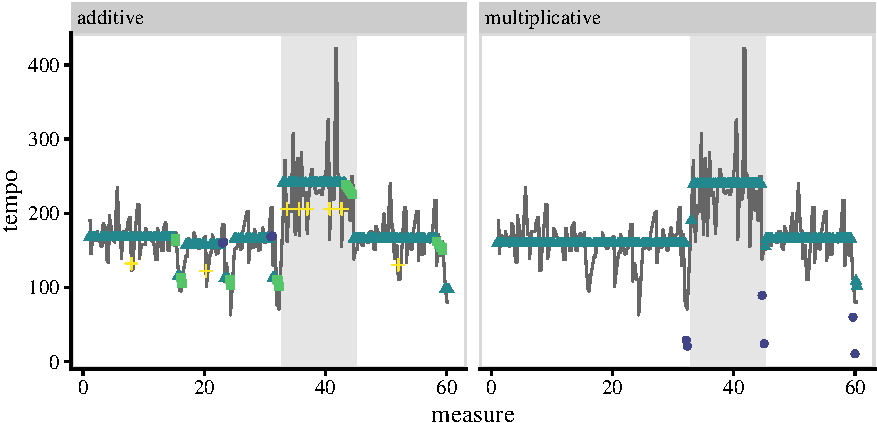
\includegraphics{Dynamics-Model_files/figure-latex/unnamed-chunk-1-1.pdf}

\newpage

\section{Estimates of Probabilities for each Performance}
\label{appendixb}

\begin{table}[H]
\centering
\begin{tabular}{lrrrr}
\toprule
  & $p_{21}$ & $p_{23}$ & $p_{24}$ & $p_{41}$\\
\midrule
\rowcolor{gray!6}  Bacha 1997 & 0.03 & 0.02 & 0.03 & 0.08\\
Barbosa 1983 & 0.02 & 0.02 & 0.02 & 0.12\\
\rowcolor{gray!6}  Biret 1990 & 0.03 & 0.04 & 0.03 & 0.12\\
Block 1995 & 0.10 & 0.03 & 0.03 & 0.12\\
\rowcolor{gray!6}  Brailowsky 1960 & 0.05 & 0.03 & 0.09 & 0.04\\
\addlinespace
Chiu 1999 & 0.04 & 0.02 & 0.03 & 0.07\\
\rowcolor{gray!6}  Clidat 1994 & 0.05 & 0.02 & 0.04 & 0.06\\
Cohen 1997 & 0.05 & 0.02 & 0.05 & 0.08\\
\rowcolor{gray!6}  Cortot 1951 & 0.03 & 0.01 & 0.06 & 0.29\\
Csalog 1996 & 0.02 & 0.02 & 0.01 & 0.14\\
\addlinespace
\rowcolor{gray!6}  Czerny-Stefanska 1990 & 0.09 & 0.02 & 0.02 & 0.15\\
Ezaki 2006 & 0.02 & 0.02 & 0.06 & 0.08\\
\rowcolor{gray!6}  Ferenczy 1958 & 0.03 & 0.04 & 0.05 & 0.08\\
Fliere 1977 & 0.03 & 0.01 & 0.02 & 0.21\\
\rowcolor{gray!6}  Fou 1978 & 0.05 & 0.02 & 0.03 & 0.09\\
\addlinespace
Francois 1956 & 0.03 & 0.03 & 0.02 & 0.08\\
\rowcolor{gray!6}  Grinberg 1951 & 0.07 & 0.03 & 0.03 & 0.08\\
Hatto 1993 & 0.06 & 0.07 & 0.07 & 0.05\\
\rowcolor{gray!6}  Hatto 2006 & 0.05 & 0.04 & 0.07 & 0.05\\
Indjic 1988 & 0.03 & 0.07 & 0.06 & 0.04\\
\addlinespace
\rowcolor{gray!6}  Jonas 1947 & 0.06 & 0.04 & 0.02 & 0.10\\
Kapell 1951 & 0.06 & 0.02 & 0.03 & 0.05\\
\rowcolor{gray!6}  Kiepura 1999 & 0.03 & 0.02 & 0.02 & 0.14\\
\bottomrule
\end{tabular}
\end{table}

\newpage

\begin{table}[H]
\centering
\begin{tabular}{lrrrr}
\toprule
  & $p_{21}$ & $p_{23}$ & $p_{24}$ & $p_{41}$\\
\midrule
\rowcolor{gray!6}  Kushner 1989 & 0.04 & 0.01 & 0.04 & 0.19\\
Luisada 1991 & 0.04 & 0.02 & 0.02 & 0.14\\
\rowcolor{gray!6}  Lushtak 2004 & 0.08 & 0.06 & 0.04 & 0.05\\
Meguri 1997 & 0.03 & 0.01 & 0.02 & 0.06\\
\rowcolor{gray!6}  Milkina 1970 & 0.05 & 0.03 & 0.02 & 0.28\\
\addlinespace
Mohovich 1999 & 0.05 & 0.02 & 0.02 & 0.11\\
\rowcolor{gray!6}  Ohlsson 1999 & 0.06 & 0.03 & 0.02 & 0.09\\
Olejniczac 1990 & 0.05 & 0.02 & 0.07 & 0.07\\
\rowcolor{gray!6}  Rangell 2001 & 0.04 & 0.01 & 0.06 & 0.05\\
Richter 1976 & 0.05 & 0.02 & 0.05 & 0.04\\
\addlinespace
\rowcolor{gray!6}  Rubinstein 1939 & 0.09 & 0.02 & 0.12 & 0.04\\
Rubinstein 1952 & 0.05 & 0.02 & 0.02 & 0.13\\
\rowcolor{gray!6}  Rubinstein 1961 & 0.04 & 0.02 & 0.03 & 0.05\\
Rubinstein 1966 & 0.03 & 0.02 & 0.02 & 0.21\\
\rowcolor{gray!6}  Shebanova 2002 & 0.05 & 0.03 & 0.07 & 0.03\\
\addlinespace
Smidowicz 1948a & 0.04 & 0.02 & 0.05 & 0.05\\
\rowcolor{gray!6}  Smidowicz 1948b & 0.05 & 0.02 & 0.07 & 0.03\\
Smith 1975 & 0.06 & 0.02 & 0.06 & 0.12\\
\rowcolor{gray!6}  Sofronitsky 1949 & 0.06 & 0.01 & 0.02 & 0.10\\
Sztompka 1959 & 0.05 & 0.02 & 0.07 & 0.03\\
\addlinespace
\rowcolor{gray!6}  Tomsic 1995 & 0.09 & 0.02 & 0.02 & 0.11\\
Uninsky 1971 & 0.05 & 0.02 & 0.07 & 0.03\\
\rowcolor{gray!6}  Wasowski 1980 & 0.03 & 0.02 & 0.02 & 0.14\\
\bottomrule
\end{tabular}
\end{table}

\includegraphics{Dynamics-Model_files/figure-latex/unnamed-chunk-3-1.pdf}

\section{Plots for each Performance}
\label{appendixd}

\includegraphics{Dynamics-Model_files/figure-latex/unnamed-chunk-4-1.pdf}
\includegraphics{Dynamics-Model_files/figure-latex/unnamed-chunk-4-2.pdf}
\includegraphics{Dynamics-Model_files/figure-latex/unnamed-chunk-4-3.pdf}
\includegraphics{Dynamics-Model_files/figure-latex/unnamed-chunk-4-4.pdf}
\includegraphics{Dynamics-Model_files/figure-latex/unnamed-chunk-4-5.pdf}
\includegraphics{Dynamics-Model_files/figure-latex/unnamed-chunk-4-6.pdf}
\includegraphics{Dynamics-Model_files/figure-latex/unnamed-chunk-4-7.pdf}
\includegraphics{Dynamics-Model_files/figure-latex/unnamed-chunk-4-8.pdf}
\includegraphics{Dynamics-Model_files/figure-latex/unnamed-chunk-4-9.pdf}
\includegraphics{Dynamics-Model_files/figure-latex/unnamed-chunk-4-10.pdf}
\includegraphics{Dynamics-Model_files/figure-latex/unnamed-chunk-4-11.pdf}
\includegraphics{Dynamics-Model_files/figure-latex/unnamed-chunk-4-12.pdf}
\includegraphics{Dynamics-Model_files/figure-latex/unnamed-chunk-4-13.pdf}
\includegraphics{Dynamics-Model_files/figure-latex/unnamed-chunk-4-14.pdf}
\includegraphics{Dynamics-Model_files/figure-latex/unnamed-chunk-4-15.pdf}
\includegraphics{Dynamics-Model_files/figure-latex/unnamed-chunk-4-16.pdf}
\includegraphics{Dynamics-Model_files/figure-latex/unnamed-chunk-4-17.pdf}
\includegraphics{Dynamics-Model_files/figure-latex/unnamed-chunk-4-18.pdf}
\includegraphics{Dynamics-Model_files/figure-latex/unnamed-chunk-4-19.pdf}
\includegraphics{Dynamics-Model_files/figure-latex/unnamed-chunk-4-20.pdf}
\includegraphics{Dynamics-Model_files/figure-latex/unnamed-chunk-4-21.pdf}
\includegraphics{Dynamics-Model_files/figure-latex/unnamed-chunk-4-22.pdf}
\includegraphics{Dynamics-Model_files/figure-latex/unnamed-chunk-4-23.pdf}
\includegraphics{Dynamics-Model_files/figure-latex/unnamed-chunk-4-24.pdf}
\includegraphics{Dynamics-Model_files/figure-latex/unnamed-chunk-4-25.pdf}
\includegraphics{Dynamics-Model_files/figure-latex/unnamed-chunk-4-26.pdf}
\includegraphics{Dynamics-Model_files/figure-latex/unnamed-chunk-4-27.pdf}
\includegraphics{Dynamics-Model_files/figure-latex/unnamed-chunk-4-28.pdf}
\includegraphics{Dynamics-Model_files/figure-latex/unnamed-chunk-4-29.pdf}
\includegraphics{Dynamics-Model_files/figure-latex/unnamed-chunk-4-30.pdf}
\includegraphics{Dynamics-Model_files/figure-latex/unnamed-chunk-4-31.pdf}
\includegraphics{Dynamics-Model_files/figure-latex/unnamed-chunk-4-32.pdf}
\includegraphics{Dynamics-Model_files/figure-latex/unnamed-chunk-4-33.pdf}
\includegraphics{Dynamics-Model_files/figure-latex/unnamed-chunk-4-34.pdf}
\includegraphics{Dynamics-Model_files/figure-latex/unnamed-chunk-4-35.pdf}
\includegraphics{Dynamics-Model_files/figure-latex/unnamed-chunk-4-36.pdf}
\includegraphics{Dynamics-Model_files/figure-latex/unnamed-chunk-4-37.pdf}
\includegraphics{Dynamics-Model_files/figure-latex/unnamed-chunk-4-38.pdf}
\includegraphics{Dynamics-Model_files/figure-latex/unnamed-chunk-4-39.pdf}
\includegraphics{Dynamics-Model_files/figure-latex/unnamed-chunk-4-40.pdf}
\includegraphics{Dynamics-Model_files/figure-latex/unnamed-chunk-4-41.pdf}
\includegraphics{Dynamics-Model_files/figure-latex/unnamed-chunk-4-42.pdf}
\includegraphics{Dynamics-Model_files/figure-latex/unnamed-chunk-4-43.pdf}
\includegraphics{Dynamics-Model_files/figure-latex/unnamed-chunk-4-44.pdf}
\includegraphics{Dynamics-Model_files/figure-latex/unnamed-chunk-4-45.pdf}
\includegraphics{Dynamics-Model_files/figure-latex/unnamed-chunk-4-46.pdf}

\bibliographystyle{agsm}
\bibliography{musicdynamicsbib.bib}

\end{document}
